\chapter{总体设计}
%==================================================================
\section{软件描述}
    系统包括前台和后台两个部分。
\subsection{前台主要功能}
    向服务器发送请求,并接受服务器的响应,向用户展示服务器的返回结果。
    
    \begin{itemize}
        \item 用户可以进行账户注册,并使用已经注册的账户登录该系统。
        \item 用户可以与其他用户进行聊天。除了基本的文字聊天,用户还可以进行音视频聊天。此外,用户可以查看自己的聊天记录。
        \item 用户可以在群聊中发言。如果身份是管理员或群主,用户还可以对群聊进行管理。此外,不同的群聊情境还会提供不同的额外群聊功能。
        \item 用户可以对自己的通讯录进行管理:可以添加或删除好友,在添加好友时系统会进行个性化推荐;可以加入或退出群聊;可以将其他用户移入或移出黑名单。
        \item 用户可以对自己的Board进行管理,新建或修改日志;也可以浏览他人的Board,对他们的日志进行评论。
        \item 用户可以进行在线文档协作。
        \item 在接收到新的信息时,用户可以得到提醒。
        \item 用户在加入组织后,可以进行活动管理,自动修改所有参与者的日历。
        \item 用户可以查看并修改自己的日历。  
        \item 用户可以管理本地和云端的文件。
        \item 用户可以将账号与邮箱或设备进行绑定,以提高账户的安全性。
        \item 用户可以通过邮箱接口得知是否有新的邮件。
    \end{itemize}
    
\subsection{后台主要功能}
后台服务器接收用户发送的动作和请求,予以处理并进行响应。

服务器在接收到用户请求时,会在服务器的数据库中进行查询操作,并且进
行返回查询结果或者反馈提示信息,对于用户提交的数据(比如发布活动、修改日志等),也会存入到数据库中。对于发送的聊天信息,服务器会将其缓存到发送队列中。

%==================================================================
\section{处理流程}
    %--------------------------------------------------------------
    \subsection{总体流程}
        % 此处应当有一个图和对应的描述。
        \begin{figure}[ht]
            \centering
            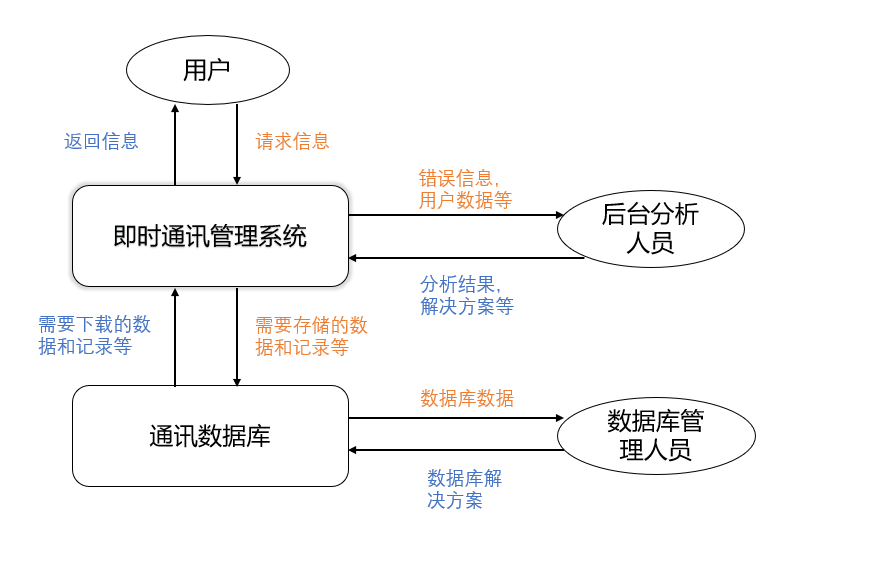
\includegraphics[scale = 0.75]{总体流程.png}\label{tab:classification}
            \caption{总体流程}\label{fig:noted-figure}
        \end{figure}
        \newpage
    %--------------------------------------------------------------
    \subsection{系统基本流程}
        % 此处应当有一个图和对应的描述。
        \begin{figure}[ht]
            \centering
            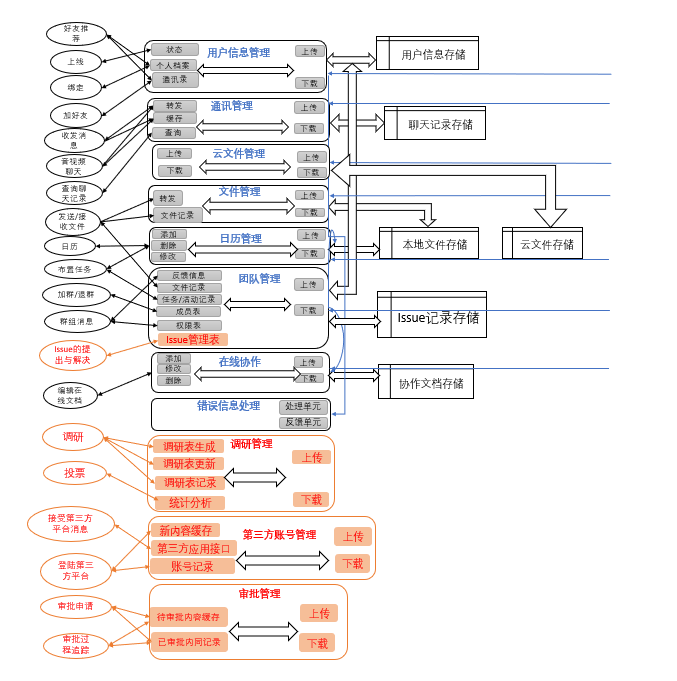
\includegraphics[scale = 0.75]{系统整体流程.png}\label{tab:classification}
            \caption{系统基本流程}\label{fig:noted-figure}
        \end{figure}
        \newpage
    %--------------------------------------------------------------
    \subsection{客户端基本流程}
        % 这只是举个例子,如果没有客户端则不需要此节。
        用户注册/登录之后,在客户端进行各种功能的调用,所有的功能在用户信息管理模块提供
        的信息下运行,接收用户操作信息,将消息提示返回给用户。
        \begin{figure}[ht]
            \centering
            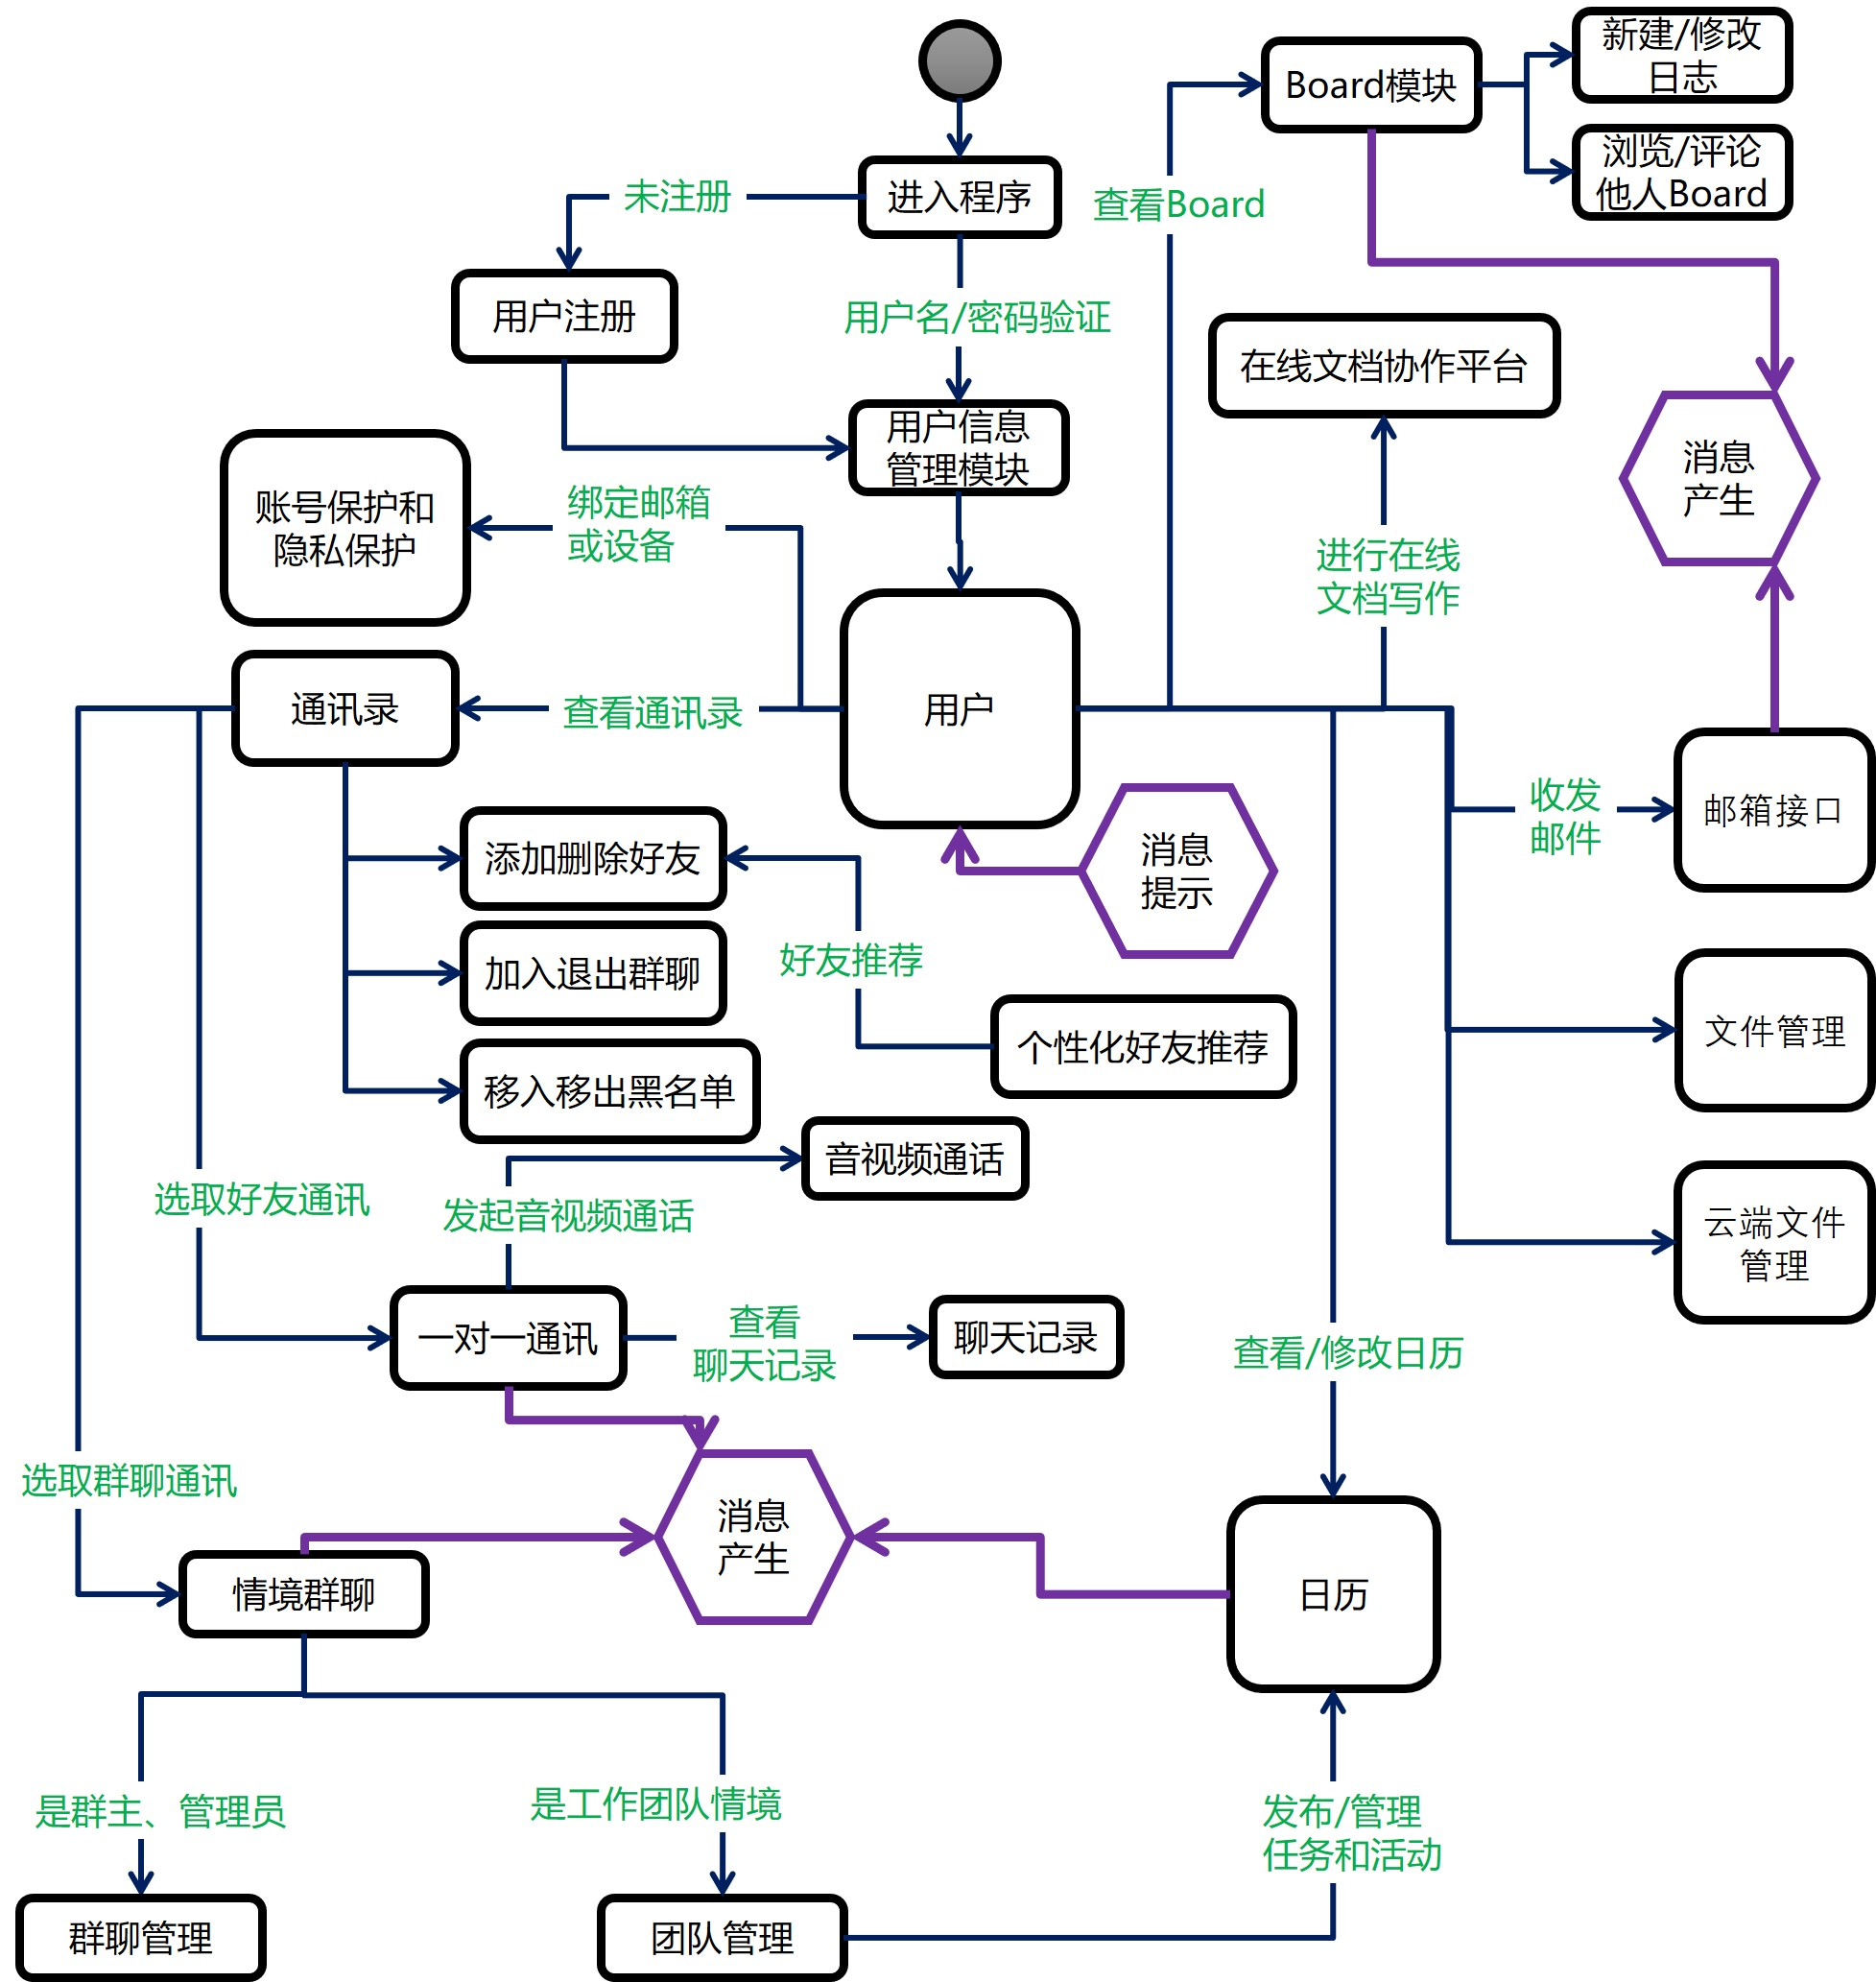
\includegraphics[scale = 0.45]{OutlineDesign/figures/客户端基本流程.jpg}
            \label{tab:classification}
            \caption{客户端基本流程}
            \label{fig:noted-figure}
        \end{figure}
        \newpage
    %--------------------------------------------------------------
    \subsection{服务器端基本流程}
    服务器端流程如图\ref{fig:server_flow}所示。
    客户端1和2展示了一对一聊天和群聊的服务器处理过程;客户端4和5展示了音视频通讯的过程;
    客户端1与服务器间的箭头展示了查询的过程;
    客户端3与服务器间的箭头展示了更新的过程
    (许多功能都可以抽象为查询和更新,在后面会详细说明)。
    服务器使用SQL语句向数据库集群发送查询或更新请求,集群返回查询或更新的结果。
        \begin{figure}[h]
            \centering
            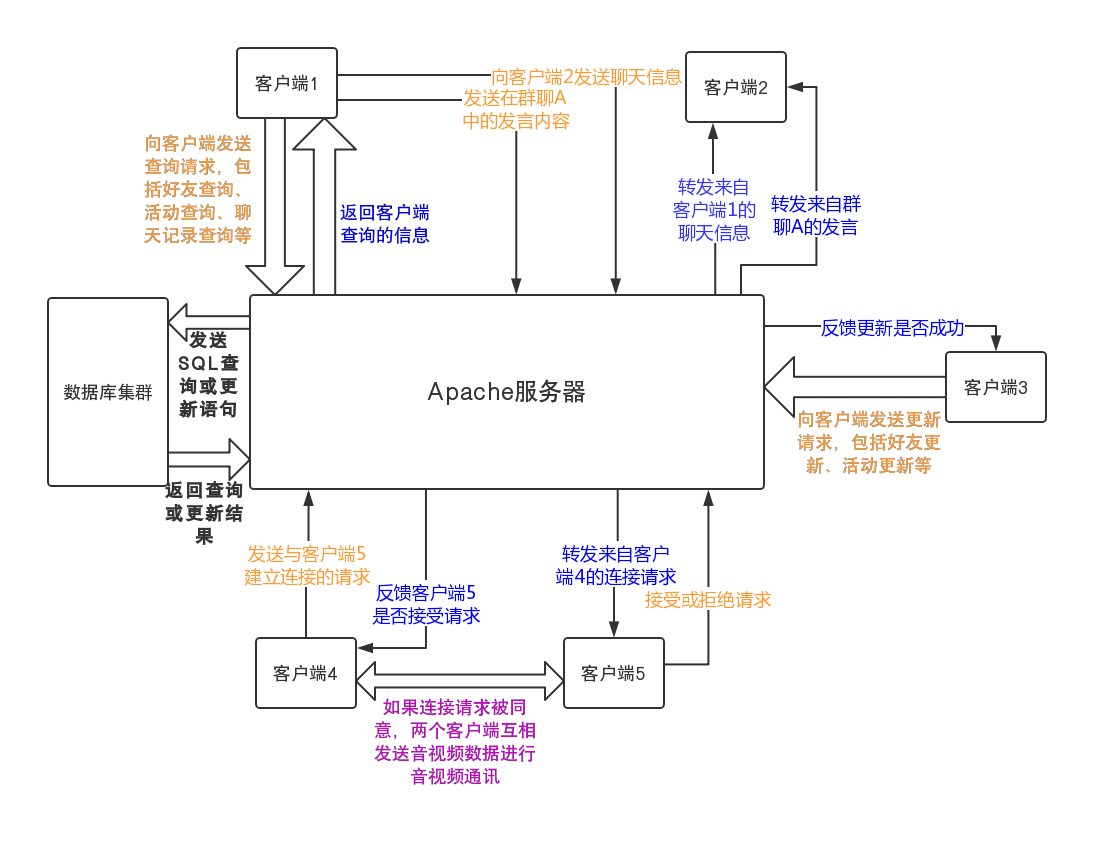
\includegraphics[scale=0.4]{OutlineDesign/figures/server_flow.png}
            \caption{服务器端流程}
            \label{fig:server_flow}
        \end{figure}
    %--------------------------------------------------------------
    \subsection{R.INTF.CALC.001: 一对一即时通讯功能·具体流程}
        \begin{enumerate}
            \item 客户端选取联系人创建对话窗口
            \item 客户端在对话窗口获取用户输入的消息
            \item 客户端向服务器端发送聊天消息,并在聊天界面上显示该消息
            \item 服务器端接收到消息后向客户端发送确认消息
            \item 客户端一段时间没有收到确认消息后,在对应的聊天消息上增加发送失败标记
            \item 如果接收用户在线,则服务器立即发送该消息;否则进行缓存,直到接收方上线再发送该消息
            \item 客户端使用监听线程接收服务器发送的消息并将消息显示给用户
            \item 客户端在聊天界面上部展示发送出和接收到的聊天信息
        \end{enumerate}
        %------------------------
        \begin{figure}[h]
            \centering
            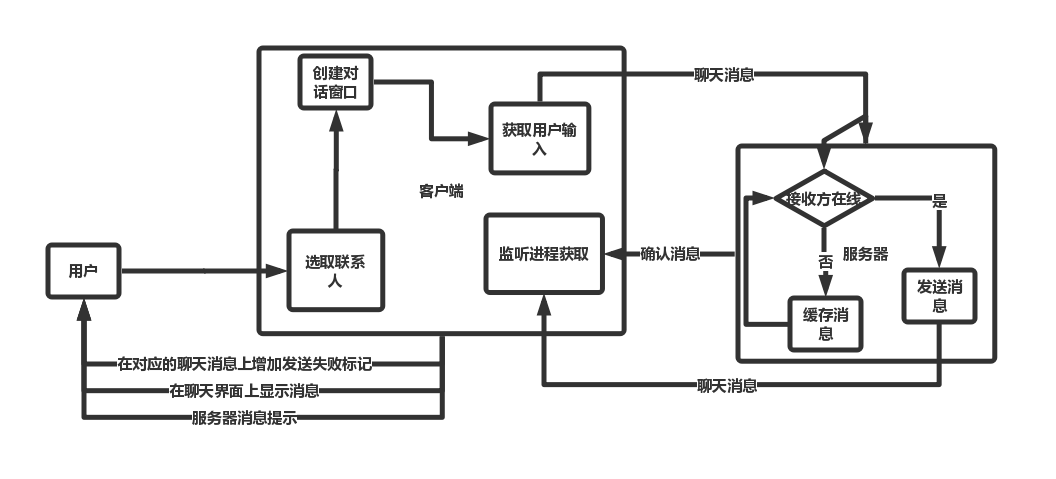
\includegraphics[scale=0.4]{OutlineDesign/figures/一对一即时通讯功能·具体流程.png}
            \caption{一对一即时通讯功能·具体流程}
            \label{fig:server_flow}
        \end{figure}
    %--------------------------------------------------------------
%================ EXAMPLE ===================================================
% 已登录用户在购物车中提交请求交易的 POST 请求,提交的表单中指明了交易中包括的
% 所有商品、商家、付款信息、收货地址,输入输出处理系统接收到合法请求后,向商品信息
% 系统请求数据,收到数据以后验证是否正确,然后向订单系统发起生成新订单的请求,订单
% 系统负责更新商品信息系统、商家信息,通知商家接单,返回订单处理结果输入输出处理系
% 统,输入输出处理系统依照结果产生 HTML 页面,并返回给用户。
%================ EXAMPLE ===================================================
    \subsection{R.INTF.CALC.002: 多情境群聊功能·具体流程}
        %--------------------------------------------------------------
        \subsubsection{R.INTF.CALC.002.1: 群管理·具体流程}
        \begin{enumerate}
            \item 用户在通讯录面板点击上方的加号按钮后选择“创建群聊”弹出群聊创建窗口,输入名称、类型等信息进行创建。
            \item 用户在通讯录面板选择已经创建的群,弹出聊天界面
            \item 在聊天界面点击“管理”按钮,弹出管理界面
            \item 用户在管理界面可以查看所有入群申请,并点击申请后的“同意”或“拒绝”按钮进行批准或拒绝
            \item 用户在管理界面可以查看所有群成员并进行“任命/解除管理员权限”或“从群聊中移除”操作
            \item 用户在管理界面可以点击“邀请”按钮邀请新成员入群
            \item 用户在管理界面可以点击“解散群聊”按钮解散该群聊
            \item 客户端对应每个操作向服务器发送请求
            \item 服务器回应是否接受请求
            \item 若接受请求,对群成员表进行相应的增删改查操作
            \item 若拒绝请求,客户端通过弹窗告知用户
            \item 客户端显示管理操作是否完成,以及完成后的群信息
        \end{enumerate}
        %------------------------
        \begin{figure}[h]
            \centering
            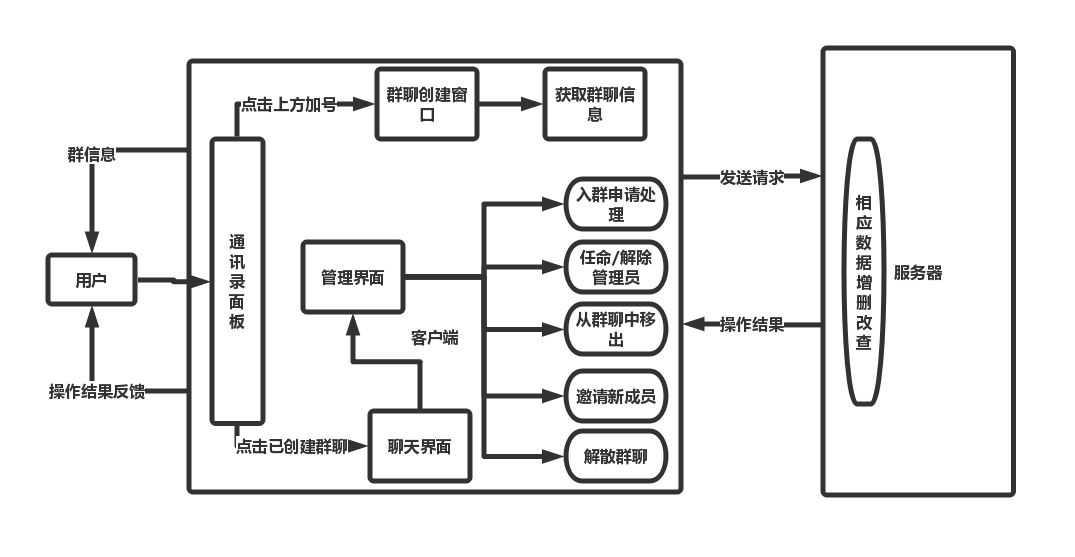
\includegraphics[scale=0.4]{OutlineDesign/figures/群管理具体流程.png}
            \caption{群管理·具体流程}
            \label{fig:server_flow}
        \end{figure}
        %--------------------------------------------------------------
        \subsubsection{R.INTF.CALC.002.2: 群聊天·具体流程}
        \begin{enumerate}
            \item 用户在通讯录中选择相应的群聊,弹出群聊窗口,在下部的对话框中输入自己的发言
            \item 客户端向服务器发送发言信息,并将该信息显示在群聊界面上部
            \item 服务器在接收到发言信息后,向客户端发送回执
            \item 如果客户端在一定时间内没有收到回执,在对应的发言信息上增加发送失败标记
            \item 服务器向所有群成员转发该信息。如果某位成员不在线,则进行缓存,直到其上线再转发该信息
            \item 客户端使用一个监听线程监听服务器,接收服务器转发的信息
            \item 客户端在群聊界面上部展示发送出的和接收到的发言信息
        \end{enumerate}
        %------------------------
        \begin{figure}[h]
            \centering
            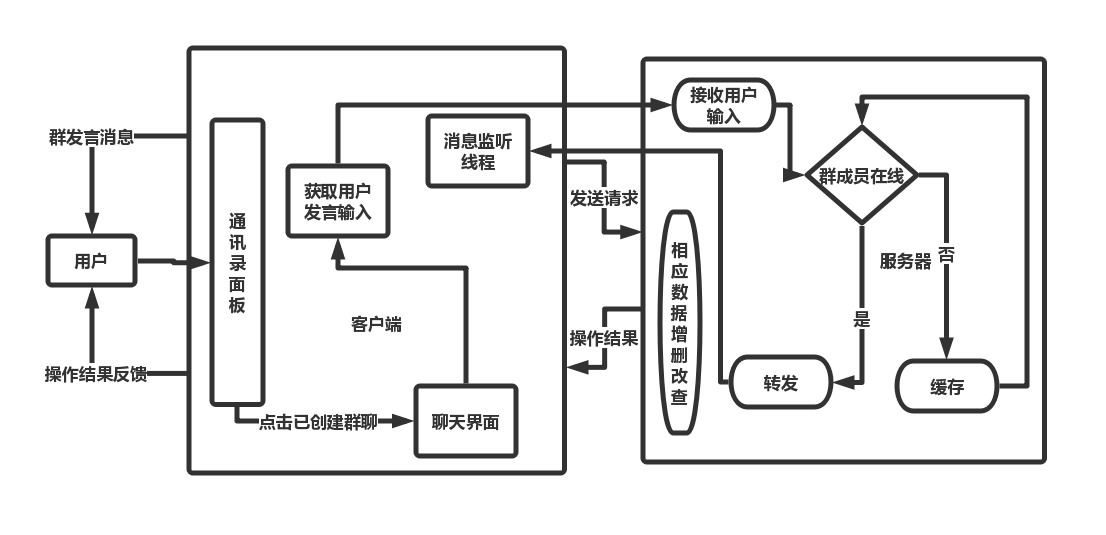
\includegraphics[scale=0.4]{OutlineDesign/figures/群聊天·具体流程.png}
            \caption{群聊天·具体流程}
            \label{fig:server_flow}
        \end{figure}
        %--------------------------------------------------------------
        \subsubsection{R.INTF.CALC.002.3: 情境功能·具体流程}
        \begin{enumerate}
            \item 用户在群聊界面点击“功能”按钮弹出功能界面
            \item 在功能界面选择各种功能,并对其进行操作,如发布和查看作业、进行签到、发布和查询成绩、更新和查看工作进度、协同写作工作汇报等
            \item 点击课程作业,调用任务管理接口
            \item 点击课堂签到,在指定时间进行GPS定位,判断用户是否位于指定地点
            \item 点击成绩查询,允许特定的用户查看成绩文件的特定部分
            \item 点击工作进度管理,调用任务管理接口
            \item 点击工作汇报协同制作,调用在线文档写作平台
            \item 在功能界面展示功能使用后的结果,如作业的内容、签到成功提示、成绩、工作完成进度、工作汇报等
        \end{enumerate}
        %------------------------
        \begin{figure}[h]
            \centering
            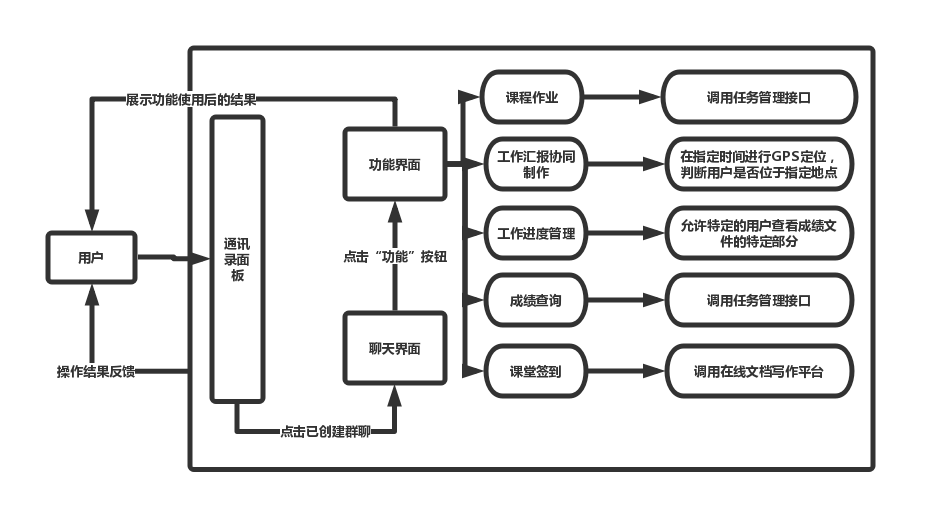
\includegraphics[scale=0.4]{OutlineDesign/figures/情境功能·具体流程.png}
            \caption{情境功能·具体流程}
            \label{fig:server_flow}
        \end{figure}
        %--------------------------------------------------------------
    \subsection{R.INTF.CALC.003: 活动/任务发布与管理功能·具体流程}
    \begin{enumerate}
        \item 用户在任务界面选择筛选和排序方式
        \item 用户在任务界面点击加号按钮,进入发布界面,设置任务的参与者、截止时间、地点、具体内容等信息并发布任务
        \item 用户点击任务后的齿轮按钮可以对该任务进行修改或删除
        \item 客户端每进行一个操作就向服务器发送一个请求,服务器返回该请求是否被接受
        \item 如果请求没有被接受,客户端通过弹窗告知用户
        \item 如果接受请求,服务器使用数据库管理所有的任务,实现增、删、改、查功能
        \item 客户端在任务界面展示任务增、删、改、查后的结果
        \item 一旦任务发生修改,客户端向用户展示任务修改的内容,可以调用邮件、短信等接口,使用电子邮件或短信来告知用户。
        \item 客户端调用日历接口,自动插入、删除、修改日历中的活动项
    \end{enumerate}
    %------------------------
        \begin{figure}[h]
            \centering
            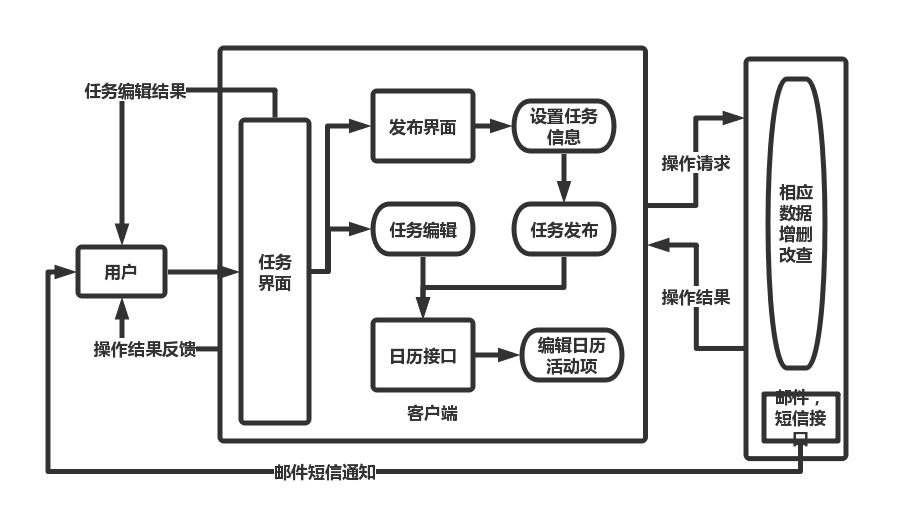
\includegraphics[scale=0.4]{OutlineDesign/figures/活动任务发布与管理功能·具体流程.png}
            \caption{活动/任务发布与管理功能·具体流程}
            \label{fig:server_flow}
        \end{figure}
    %--------------------------------------------------------------
    \subsection{R.INTF.CALC.004: 音视频通话 (会议) 功能·具体流程}
    \begin{enumerate}
        \item 用户在聊天界面点击“音频通话”或“视频通话”按钮发起连接请求
        \item 如果请求被对方拒绝,客户端则弹出窗口提示用户,停止服务
        \item 用户在聊天界面点击对方发送的连接请求后的“接受”或“拒绝”按钮接受或拒绝对方的连接请求
        \item 用户在在通话时,点击“断开”按钮停止连接
        \item 客户端权限检查:检查是否拥有所有必需的权限,如视频连接所需的摄像头权限,音频连接所需的麦克风和扬声器权限。如果缺少权限,就向用户请求对应的权限
        \item 客户端如果没有得到必需的权限,则弹出窗口提示用户,停止服务
        \item 客户端向对方发起建立连接的请求,等待对方接受
        \item 客户端调用摄像头或麦克风对用户的图像或声音进行实时录制,并发送给连接的另一方
        \item 客户端使用屏幕播放视频或扬声器播放音频,直到用户停止连接
        \item 客户端对接收到的数据进行缓存,再播放,保证播放不会乱序
        \item 如果发生用户点击按钮停止连接的事件,客户端就断开连接,停止服务
    \end{enumerate}
    %------------------------
        \begin{figure}[h]
            \centering
            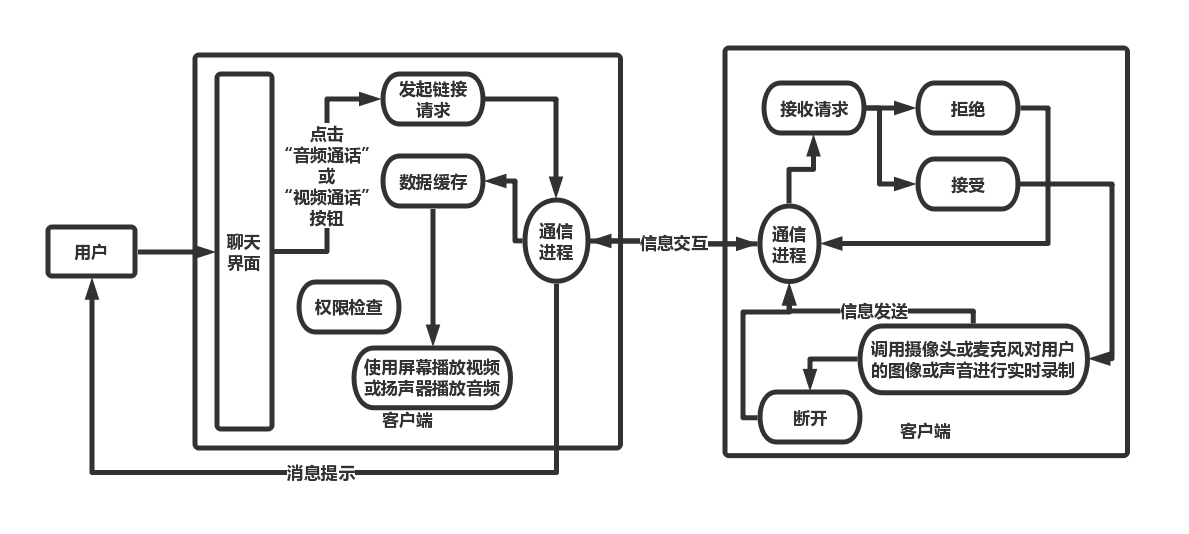
\includegraphics[scale=0.4]{OutlineDesign/figures/音视频通话会议功能·具体流程.png}
            \caption{音视频通话 (会议) 功能·具体流程}
            \label{fig:server_flow}
        \end{figure}
    %--------------------------------------------------------------
    \subsection{R.INTF.CALC.005: 通讯录功能·具体流程}
        %--------------------------------------------------------------
        \subsubsection{R.INTF.CALC.005.1: 好友管理·具体流程}
        \begin{enumerate}
            \item 用户在通讯录界面点击加号按钮后选择“添加好友”弹出好友查询界面,输入查询条件添加好友
            \item 用户在通讯录界面点击好友请求按钮展开好友请求,点击请求后的“同意”或“拒绝”按钮接受或拒绝好友请求
            \item 用户在通讯录界面上的查询框输入查询条件(好友用户名的一部分),点击“查询”按钮开始查询
            \item 用户长按某好友选择“分组”将其加入某个分组,选择“备注”为其增加备注,选择“删除”将其删除
            \item 客户端每进行一个操作就向服务器发送一个请求,服务器返回该请求是否被接受
            \item 如果请求没有被接受,客户端通过弹窗告知用户
            \item 如果接受请求,服务器使用数据库管理所有的任务,实现增、删、改、查功能
            \item 添加好友:服务器根据提供的信息定位到具体的用户,向他发送请求;在他接受后,把他的信息加入通讯录
            \item 删除好友:服务器从用户的通讯录中删除该好友,同时从他的通讯录中删除用户信息。
            \item 查询好友:服务器将用户的查询字符串与好友的用户名进行不完全字符串匹配,进行从通讯录中找到对应的好友。
            \item 备注好友:服务器为好友增加备注
            \item 好友分组:服务器在通讯录中对好友分组管理
            \item 客户端在通讯录界面主体依次列出所有的好友和群聊(如果在查询状态则列出所有符合查询条件的好友和群聊)
        \end{enumerate}
        %------------------------
        \begin{figure}[h]
            \centering
            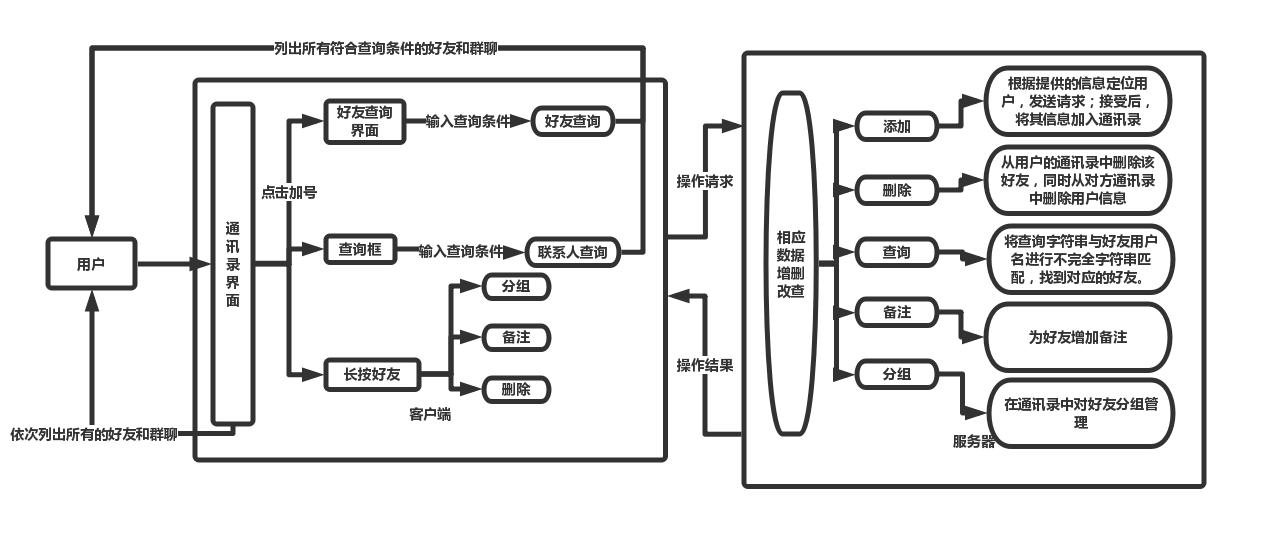
\includegraphics[scale=0.4]{OutlineDesign/figures/好友管理·具体流程.png}
            \caption{好友管理·具体流程}
            \label{fig:server_flow}
        \end{figure}
        %--------------------------------------------------------------
        \subsubsection{R.INTF.CALC.005.2: 群聊管理·具体流程}
        \begin{enumerate}
            \item 用户在通讯录界面点击加号按钮后选择“加入群聊”弹出群聊查询界面,输入查询条件加入群聊
            \item 用户在通讯录界面点击入群邀请按钮展开入群邀请,点击请求后的“同意”或“拒绝”按钮接受或拒绝入群邀请
            \item 用户在通讯录界面上的查询框输入查询条件(群聊名的一部分),点击“查询”按钮开始查询。
            \item 用户长按某群聊选择“退出”退出该群聊
            \item 客户端每进行一个操作就向服务器发送一个请求,服务器返回该请求是否被接受
            \item 如果请求没有被接受,客户端通过弹窗告知用户
            \item 如果接受请求,服务器使用数据库管理所有的任务,实现增、删、改、查功能
            \item 添加群聊:服务器根据提供的信息定位到具体的群聊,向其发送入群请求在申请被接受后,把群聊的信息加入通讯录
            \item 退出群聊:服务器从用户的通讯录中删除该群聊,同时从它的群成员中删除用户信息
            \item 查询群聊:服务器从通讯录中找到对应的群聊
            \item 客户端在通讯录界面主体依次列出所有的好友和群聊(如果在查询状态则列出所有符合查询条件的好友和群聊)
        \end{enumerate}
        %------------------------
        \newpage
        \begin{figure}[h]
            \centering
            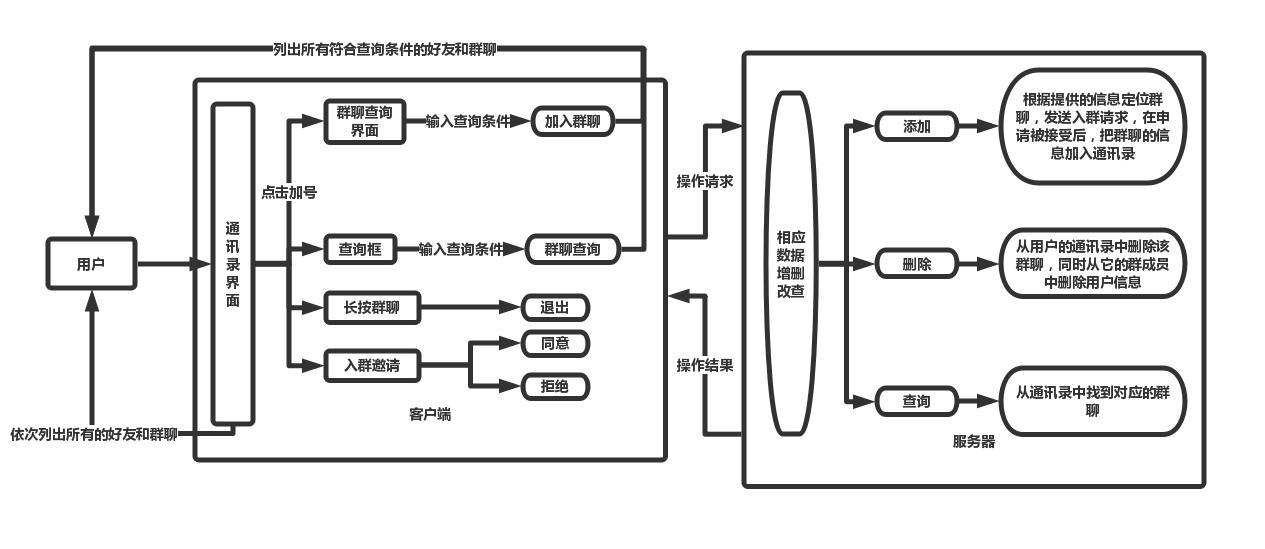
\includegraphics[scale=0.4]{OutlineDesign/figures/群聊管理·具体流程.png}
            \caption{群聊管理·具体流程}
            \label{fig:server_flow}
        \end{figure}
        %--------------------------------------------------------------
        \subsubsection{R.INTF.CALC.005.3: 黑名单·具体流程}
        \begin{enumerate}
            \item 用户长按某个好友选择“加入黑名单”将其加入黑名单
            \item 用户在通讯录界面点击“黑名单”按钮展开黑名单,长按黑名单用户并选择“移出黑名单”将其移出黑名单
            \item 客户端每进行一个操作就向服务器发送一个请求,服务器返回该请求是否被接受
            \item 如果请求没有被接受,客户端通过弹窗告知用户
            \item 如果接受请求,服务器使用数据库管理所有的任务,实现增、删、改、查功能
            \item 服务器把被选中的用户加入或移出黑名单
            \item 服务器在转发信息时,如果发送方在接收方的黑名单中,立即将该信息丢弃
            \item 客户端展示用户在上述操作后的新黑名单
        \end{enumerate}
        %------------------------
        \begin{figure}[h]
            \centering
            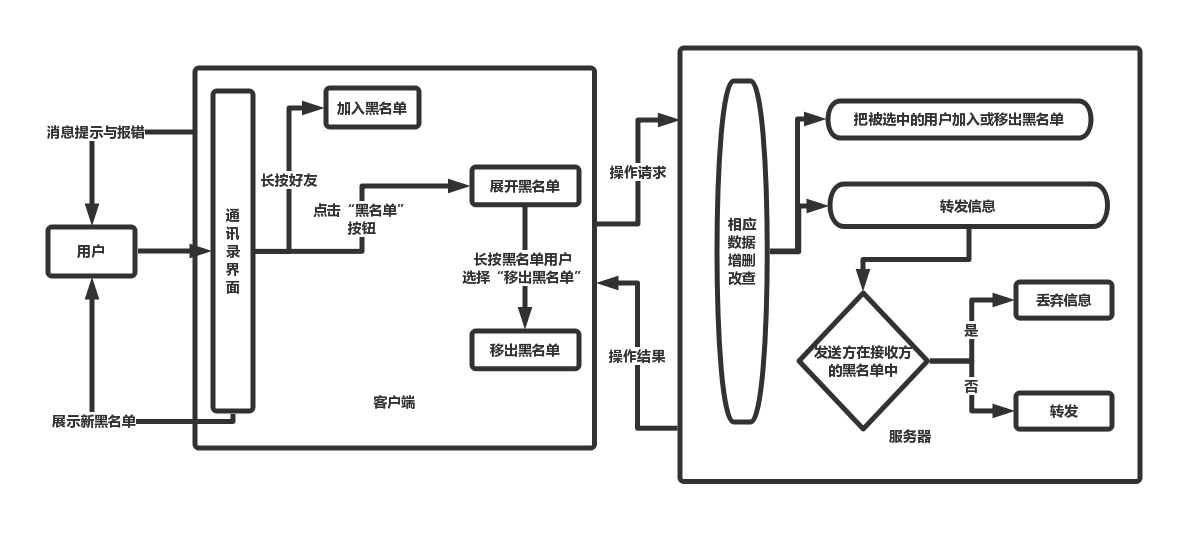
\includegraphics[scale=0.4]{OutlineDesign/figures/黑名单·具体流程.png}
            \caption{黑名单·具体流程}
            \label{fig:server_flow}
        \end{figure}
        %--------------------------------------------------------------
    \subsection{R.INTF.CALC.006: 聊天记录功能·具体流程}
    \begin{enumerate}
        \item 用户在聊天界面点击“聊天记录”按钮弹出聊天记录界面,在该界面输入查询条件(时间、聊天对象、关键词等)进行查询,点击“导出”按钮进行导出
        \item 客户端在用户聊天的同时,记录所有的聊天内容,存放在聊天记录中
        \item 客户端将聊天记录发送到服务器
        \item 服务器将聊天记录存储在云端
        \item 客户端对用户提供的查询条件,向服务器发送一个请求,检索聊天记录,返回对应的内容
        \item 客户端在导出时,将聊天记录以对应的格式写入文件
        \item 客户端在聊天记录界面向用户展示查询得到的聊天内容
        \item 客户端如果文件写入失败(目录不存在、存储已满等),弹出窗口向用户报错
    \end{enumerate}
    
    %--------------------------------------------------------------
    \subsection{R.INTF.CALC.007: 消息提醒功能·具体流程}
    \begin{enumerate}
        \item 客户端使用监听线程监听服务器发送的信息,每当有消息时发出提示声
        \item 客户端使用一个队列存储未读信息,所有接收到的消息先放入该队列,队列长度就是未读信息数目
        \item 客户端每当一条消息被读后,将它从队列移除
    \end{enumerate}
    %------------------------
        \begin{figure}[h]
            \centering
            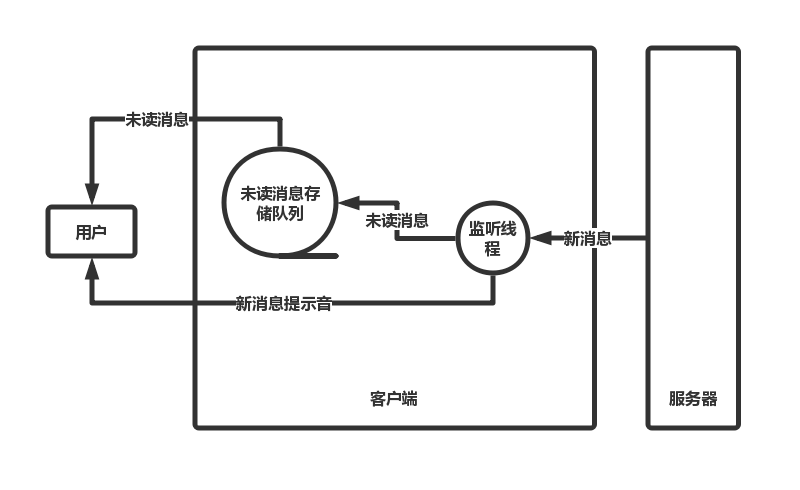
\includegraphics[scale=0.4]{OutlineDesign/figures/消息提醒功能·具体流程.png}
            \caption{消息提醒功能·具体流程}
            \label{fig:server_flow}
        \end{figure}
    %--------------------------------------------------------------
    \subsection{R.INTF.CALC.008: Board(广场) 功能·具体流程}
    \begin{enumerate}
        \item 用户点击“Board”按钮进入自己的 Board 界面
        \item 用户在Board界面点击“新建日志”新建一个日志,用户可以输入日志内容
        \item 用户在Board界面点击已经发布的日志可以进行查看,点击“评论”按钮可以进行评论,点击“删除”按钮可以将其删除
        \item 用户在 Board 界面点击好友的用户名可以跳转到他的 Board 界面
        \item 客户端每进行一个操作就向服务器发送一个请求,服务器返回该请求是否被接受
        \item 如果请求没有被接受,客户端通过弹窗告知用户
        \item 如果接受请求,服务器使用数据库管理所有的任务,实现增、删、改、查功能
        \item 服务器接收用户的输入,对 Board 进行修改
        \item 服务器在用户浏览他人的 Board 或评论他人的日志前,进行权限检查
        \item 服务器向客户端发送相应的返回信息
        \item 如果没有权限,客户端弹窗拒绝用户的浏览或评论请求
        \item 客户端在 Board 界面向用户展示日志和评论信息
    \end{enumerate}
    
    %--------------------------------------------------------------
    \subsection{R.INTF.CALC.009: 个性化好友推荐功能·具体流程}
    \begin{enumerate}
        \item 服务器根据用户聊天信息、好友信息等,利用推荐算法和社区算法得到一个用户集合
        \item 服务器从该集合中随机选出五个符合要求的用户作为推荐的好友
        \item 服务器向客户端发送推荐结果
        \item 客户端在好友查询界面,当用户没有输入查询条件时,默认展示推荐的好友
    \end{enumerate}
    %------------------------
        \begin{figure}[h]
            \centering
            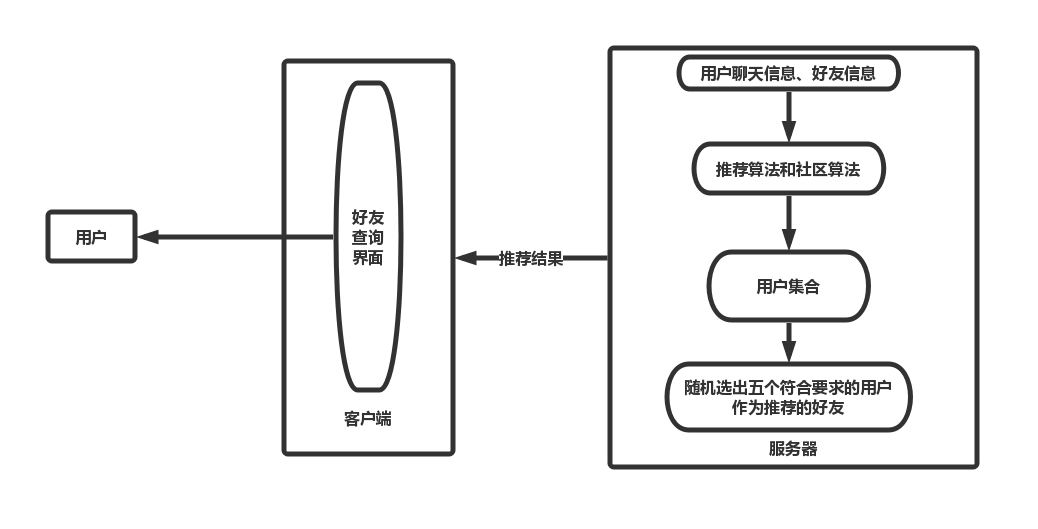
\includegraphics[scale=0.4]{OutlineDesign/figures/个性化好友推荐功能·具体流程.png}
            \caption{个性化好友推荐功能·具体流程}
            \label{fig:server_flow}
        \end{figure}
    %--------------------------------------------------------------
    \subsection{R.INTF.CALC.010: 在线文档协作平台功能·具体流程}
    \begin{enumerate}
        \item 用户点击“在线文档”按钮弹出在线文档协作平台,在该平台中可以对共享文档 进行修改
        \item 客户端每进行一个操作就向服务器发送一个请求,服务器返回该请求是否被接受
        \item 如果请求没有被接受,客户端通过弹窗告知用户
        \item 如果接受请求,服务器使用数据库管理所有的任务,实现增、删、改、查功能
        \item 服务器将在线文档存储在云端
        \item 服务器利用锁等机制,可以避免用户的修改发生冲突
        \item 客户端根据在线文档的格式,将其内容写入本地文件
        \item 客户端在在线文档协作平台向用户实时显示在线文档
    \end{enumerate}
    
    %--------------------------------------------------------------
    \subsection{R.INTF.CALC.011: 账号保护和隐私保护功能·具体流程}
    \begin{enumerate}
        \item 用户绑定邮箱、设备
        \item 客户端每进行一个操作就向服务器发送一个请求,服务器返回该请求是否被接受
        \item 如果请求没有被接受,客户端通过弹窗告知用户
        \item 如果接受请求,服务器使用数据库管理所有的任务,实现增、删、改、查功能
        \item 服务器将邮箱与账号进行绑定,在修改密码等敏感操作时必须通过邮箱进行验证
        \item 服务器将邮箱与设备绑定,在未绑定的设备上登录时必须使用绑定设备验证
        \item 服务器如果绑定成功,客户端提示绑定成功;否则,客户端提示绑定失败
    \end{enumerate}
    %------------------------
        \begin{figure}[h]
            \centering
            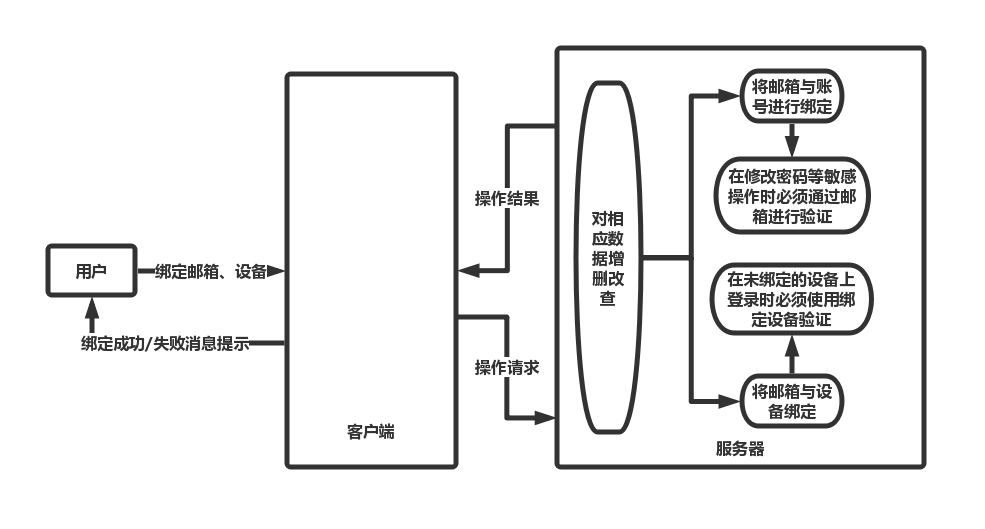
\includegraphics[scale=0.4]{OutlineDesign/figures/账号保护和隐私保护功能·具体流程.png}
            \caption{账号保护和隐私保护功能·具体流程}
            \label{fig:server_flow}
        \end{figure}
    %--------------------------------------------------------------
    \subsection{R.INTF.CALC.012: 日历管理功能·具体流程}
    \begin{enumerate}
        \item 用户点击“日历”按钮可以进入日历界面,在该界面点击具体的日期可以显示当天的活动项列表
        \item 用户在活动项列表界面,点击加号按钮可以增加新的活动项
        \item 用户在活动项列表界面,长按已经存在的活动并选择编辑可以进行修改,选择删除可以将其删除
        \item 客户端每进行一个操作就向服务器发送一个请求,服务器返回该请求是否被接受
        \item 如果请求没有被接受,客户端通过弹窗告知用户
        \item 如果接受请求,服务器使用数据库管理所有的任务,实现增、删、改、查功能
        \item 客户端在活动的时间到达时,调用消息提醒接口,对用户进行提醒
        \item 客户端在日历界面展示日历,点击日历中具体的一天可以显示当天的活动项
    \end{enumerate}
     %------------------------
        \begin{figure}[h]
            \centering
            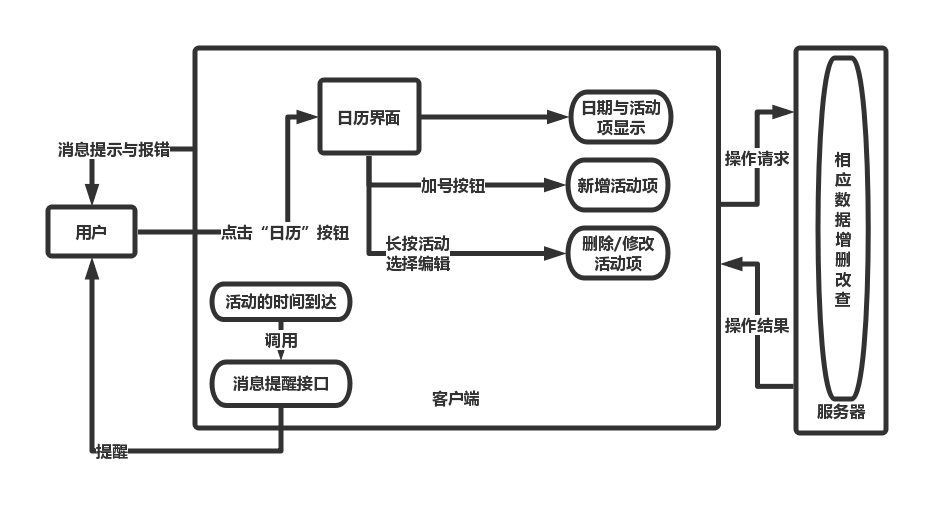
\includegraphics[scale=0.4]{OutlineDesign/figures/日历管理功能·具体流程.png}
            \caption{日历管理功能·具体流程}
            \label{fig:server_flow}
        \end{figure}
    %--------------------------------------------------------------
    \subsection{R.INTF.CALC.013: 个人本地和云端文件管理功能·具体流程}
    \begin{enumerate}
        \item 用户将需要发送的文件拖入聊天界面的对话框进行发送
        \item 客户端每进行一个操作就向服务器发送一个请求,服务器返回该请求是否被接受
        \item 如果请求没有被接受,客户端通过弹窗告知用户
        \item 如果接受请求,服务器使用数据库管理所有的任务,实现增、删、改、查功能
        \item 服务器对所有的文件进行云端存储。
        \item 服务器定期删除过期的云端文件
        \item 客户端将用户接收的文件保存在本地
        \item 如果云存储空间不足,客户端提示用户扩容
        \item 如果本地存储空间不足,客户端向用户报错
    \end{enumerate}
    %------------------------
        \begin{figure}[h]
            \centering
            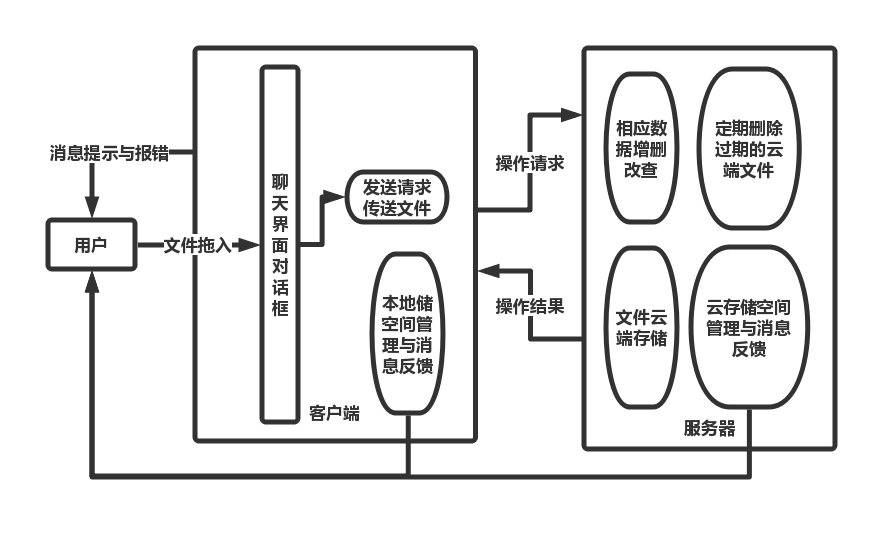
\includegraphics[scale=0.4]{OutlineDesign/figures/个人本地和云端文件管理功能·具体流程.png}
            \caption{个人本地和云端文件管理功能·具体流程}
            \label{fig:server_flow}
        \end{figure}
    %--------------------------------------------------------------
    \subsection{R.INTF.CALC.014: 邮箱接口功能·具体流程}
    \begin{enumerate}
        \item 用户在设置界面输入邮箱地址以绑定邮箱
        \item 客户端每进行一个操作就向服务器发送一个请求,服务器返回该请求是否被接受
        \item 如果请求没有被接受,客户端通过弹窗告知用户
        \item 如果接受请求,服务器使用数据库管理所有的任务,实现增、删、改、查功能
        \item 服务器在账户信息中增加一个条目,存储绑定的电子邮箱
        \item 客户端通过第三方查询绑定的电子邮箱是否有邮件,一旦有邮件就调用消息提醒接口进行提醒
    \end{enumerate}
     %------------------------
        \begin{figure}[h]
            \centering
            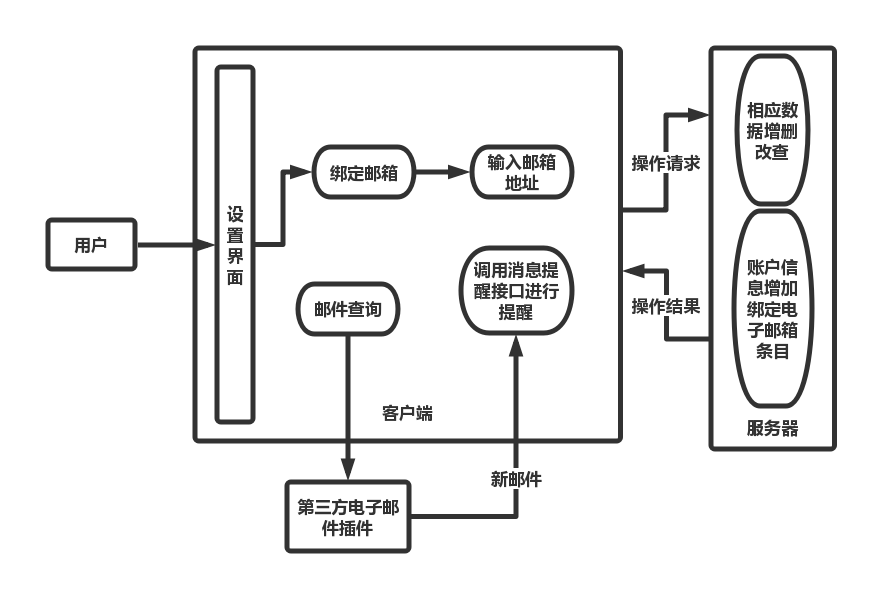
\includegraphics[scale=0.4]{OutlineDesign/figures/邮箱接口功能·具体流程.png}
            \caption{邮箱接口功能·具体流程}
            \label{fig:server_flow}
        \end{figure}
    %--------------------------------------------------------------
%==================================================================
\section{功能结构设计}
    %--------------------------------------------------------------
    \subsection{整体结构}
        即时通讯系统的整体结构为客户端前端————服务器————Oracle数据库架构,三个子系统
        分别部署不同的功能,可以相邻地进行通讯。
        \begin{figure}[h]
            \centering
            
\includegraphics[scale=0.4]{OutlineDesign/figures/整体结构.png}
            \caption{整体结构}
            \label{fig:server_flow}
        \end{figure}
%============================== GUIDE ========================================
% 此处应当有一个图和对应的描述。系统如果像微内核那样,划分成核心模块和若干个子
% 系统,此处应当有图示及说明,然后后续几个节应当描述这几个子系统。如果系统像宏
% 内核,那应当说明有哪些紧密联系的模块,并在后续几个节内描述这些模块。
%============================== GUIDE ========================================
    \subsection{客户端结构}
%============================== GUIDE ========================================
% 此处应当有一个图和对应的描述。这只是举个例子。可能的内容包括用户端的具体模
% 块、耦合情况等。
%============================== GUIDE ========================================
        客户端前端是与用户交互的主要界面,需要对所有的为用户提供的功能进行美观、
        结构和高效的管理组织与实现,具体功能结构如下图:
        \newpage
        \begin{figure}[h]
            \centering
            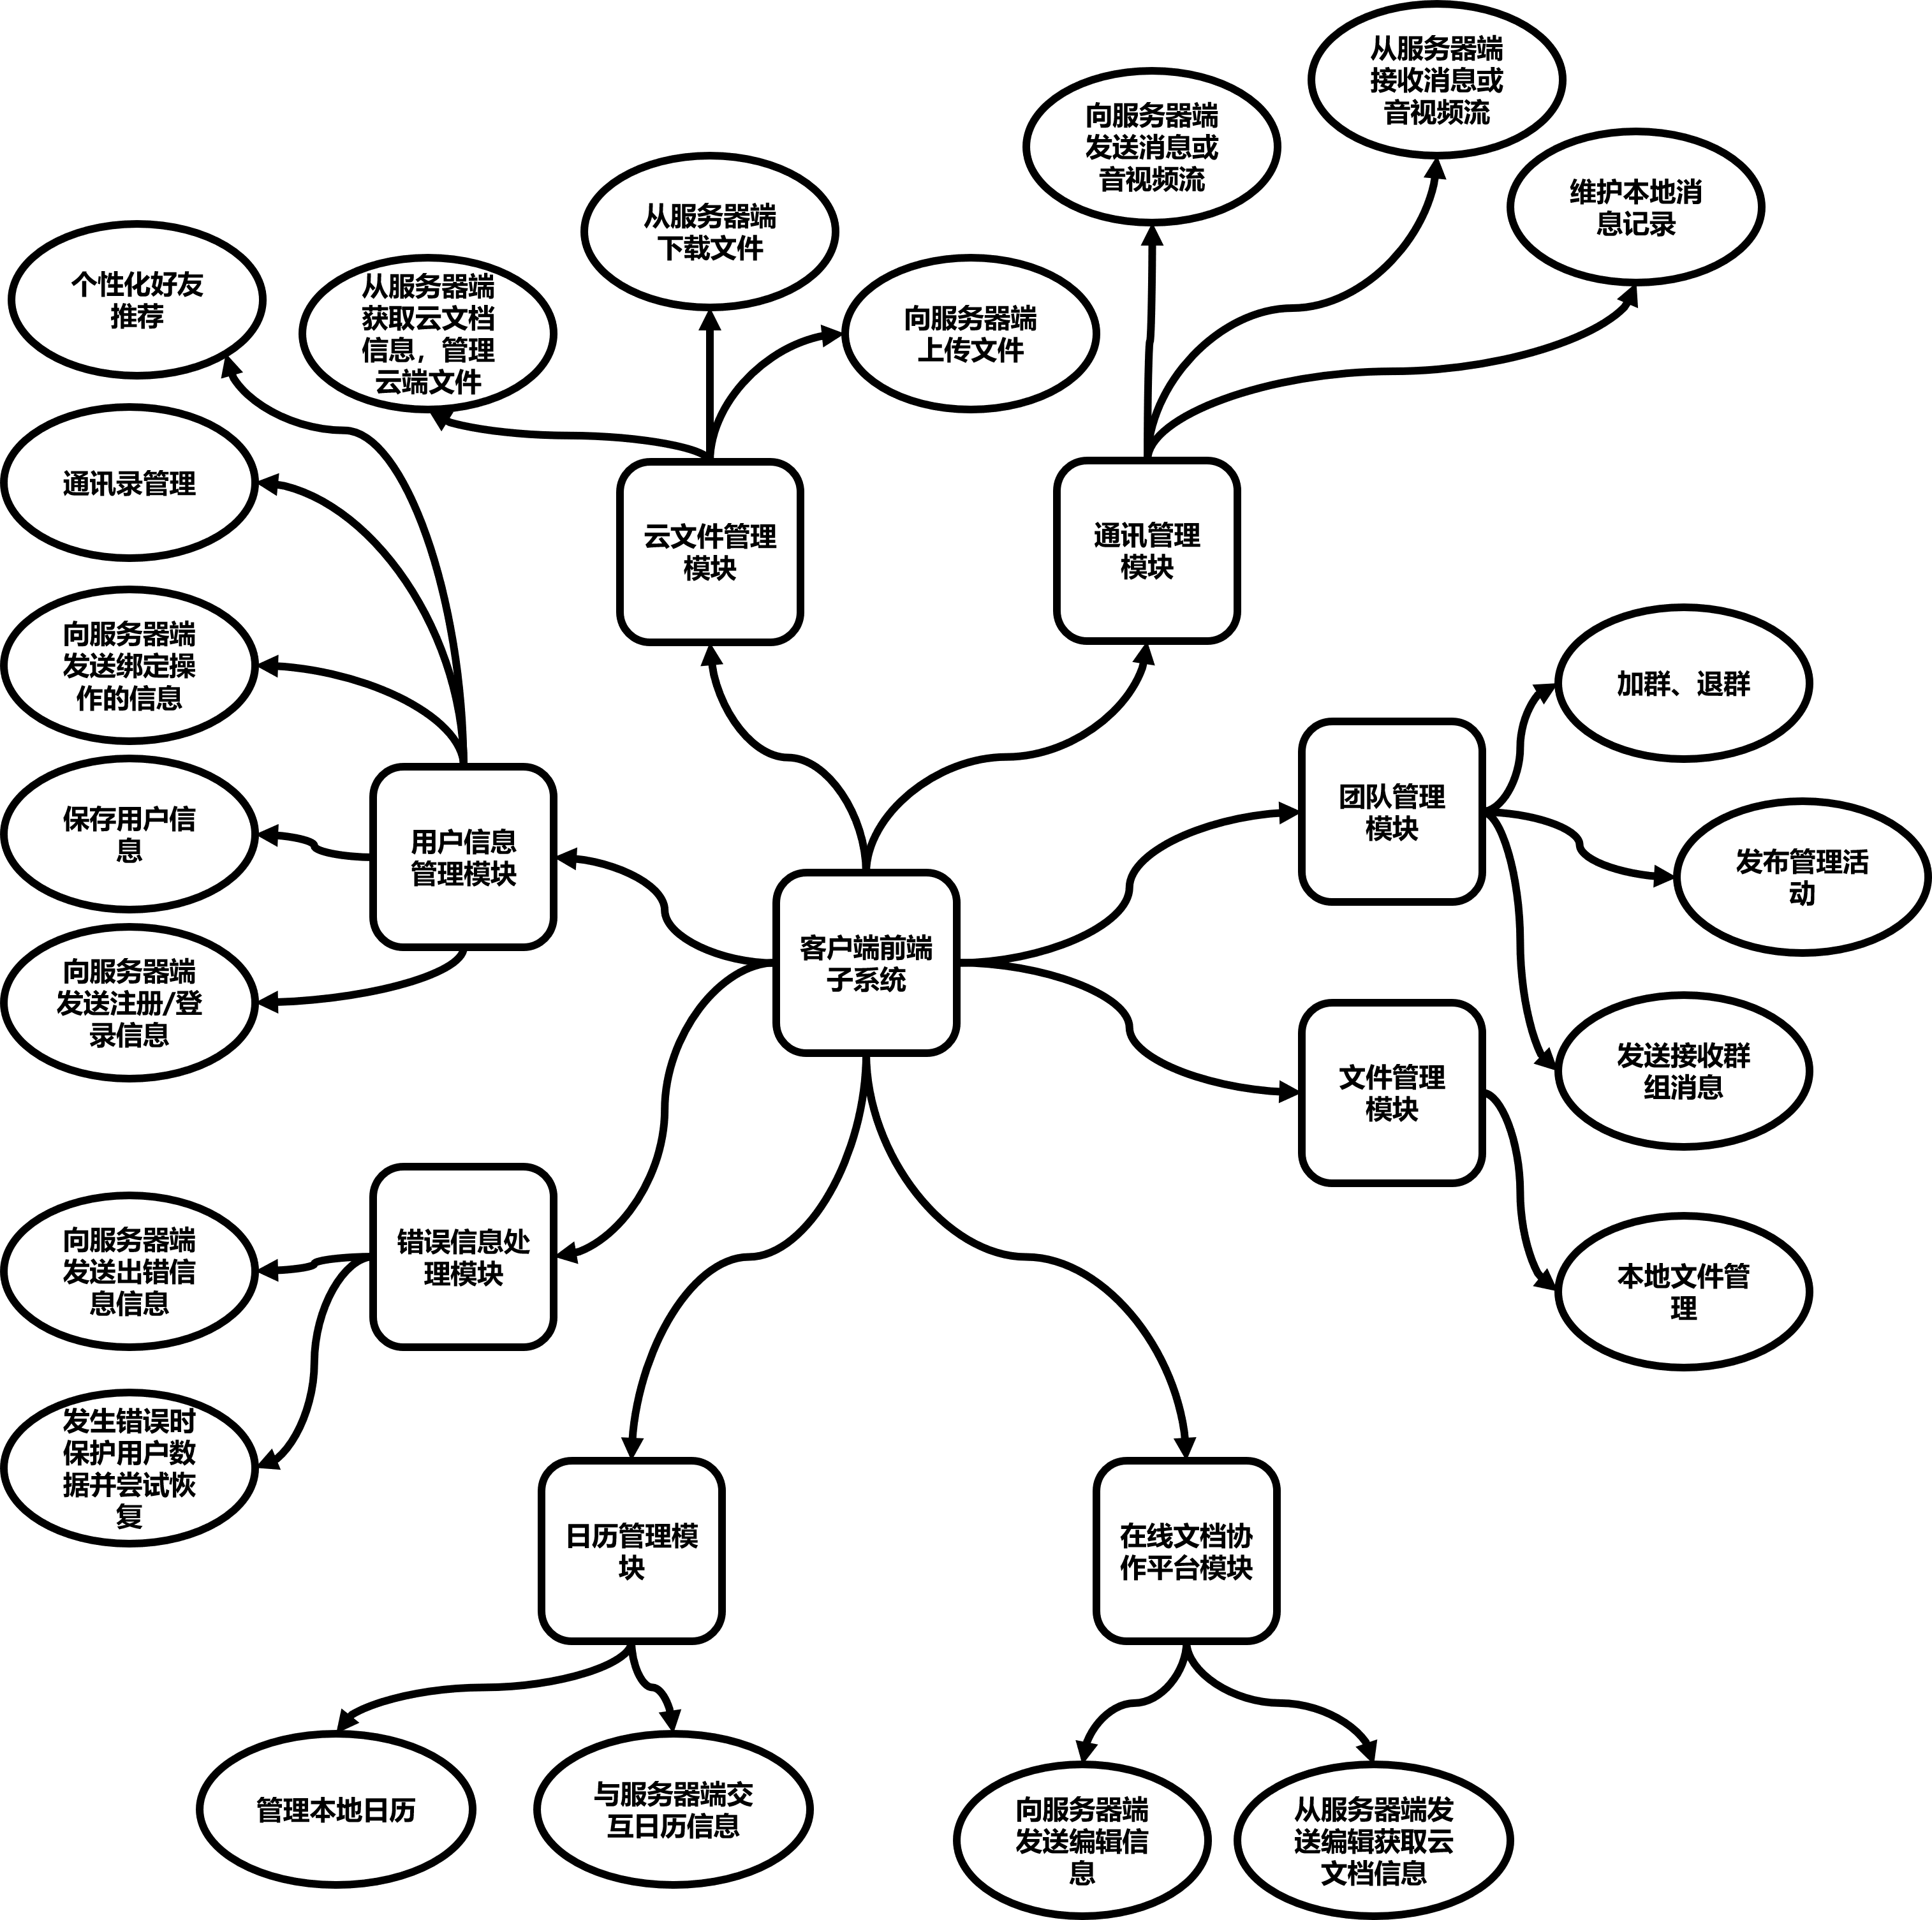
\includegraphics[scale=0.25]{OutlineDesign/figures/用户端结构.png}
            \caption{用户端结构}
            \label{fig:server_flow}
        \end{figure}
    \subsection{服务器端结构}
    
%============================== GUIDE ========================================
% 此处应当有一个图和对应的描述。这只是举个例子
        \newpage
        \begin{figure}[h]
            \centering
            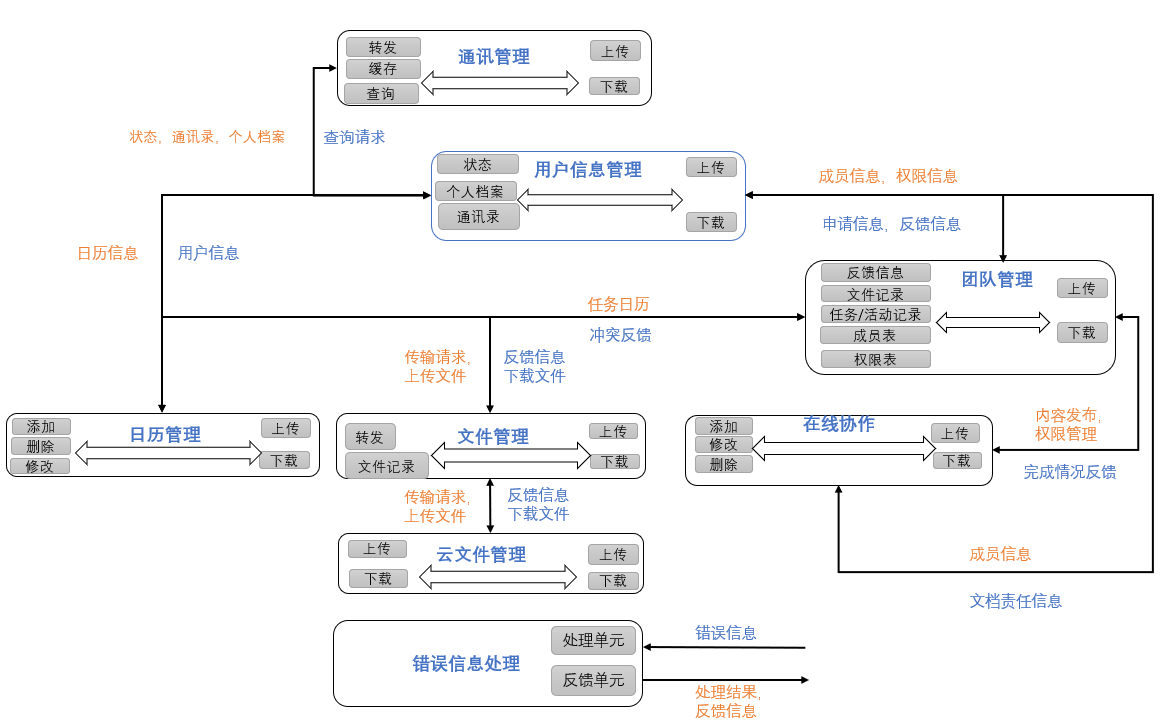
\includegraphics[scale=0.65]{OutlineDesign/figures/服务器端功能结构.png}
            \caption{服务器端功能结构}
            \label{fig:server_flow}
        \end{figure}。
%============================== GUIDE ========================================
    
    \subsection{后台数据库维护模块结构}
%============================== GUIDE ========================================
% 此处应当有一个图和对应的描述。这只是举个例子。
\newpage
        \begin{figure}[h]
            \centering
            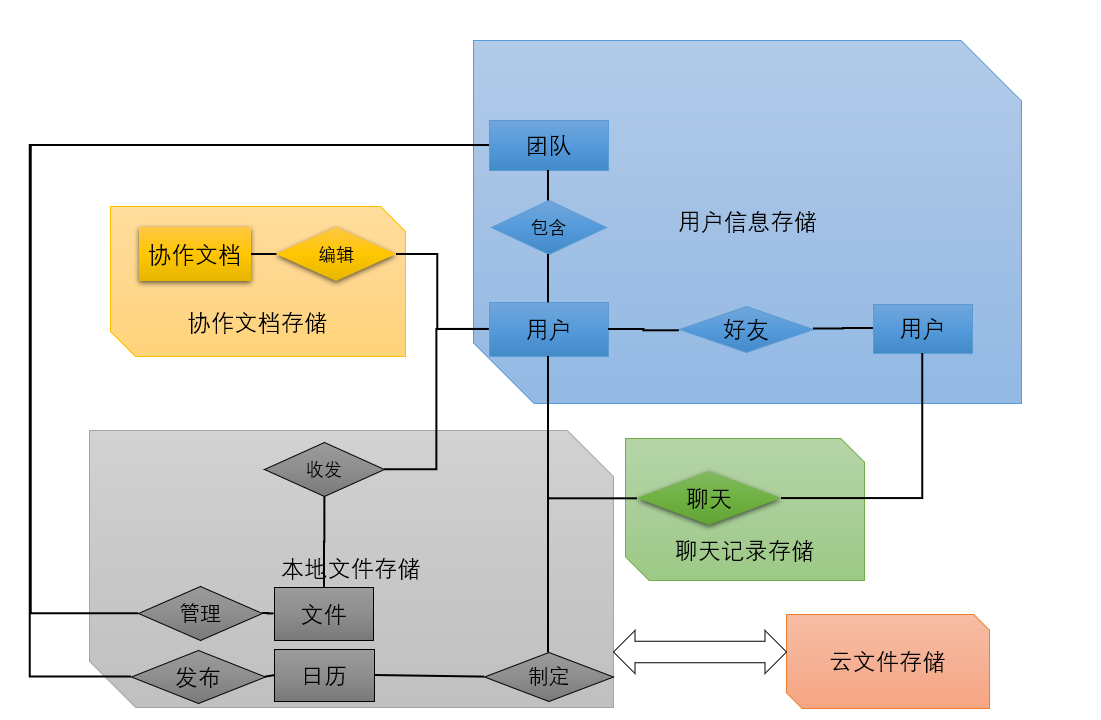
\includegraphics[scale=0.75]{OutlineDesign/figures/数据库存储结构.png}
            \caption{后台数据库维护模块结构}
            \label{fig:server_flow}
        \end{figure}
%============================== GUIDE ========================================
    
%==================================================================
\section{功能需求与程序代码的关系}
%============================== GUIDE ========================================
% [此处指的是不同的需求分配到哪些模块去实现。可按不同的端拆分此表]
%============================== GUIDE ========================================
    \begin{table}[htbp]
        \centering
        \small
        \caption{功能需求与程序代码的关系表} \label{tab:requirement-module}
            \begin{tabular}{|p{9em}|p{2.5em}|p{2.5em}|p{2.5em}|p{2.5em}|p{2.5em}|
                            p{2.5em}|p{2.5em}|p{2.5em}|}
            \hline %**********************************************************
            ·   & 用户信息管理模块      & 错误信息处理模块  & 云文件管理模块 
                & 文件管理模块          & 日历管理模块      & 团队管理模块      
                & 在线文档协作平台模块  & 通讯管理模块\\
            \hline %**********************************************************
            R.INTF.CALC.001: 一对一即时通讯功能
            %   & 用户信息管理模块      & 错误信息处理模块  & 云文件管理模块 
                & Y                     & Y                 & · 
            %   & 文件管理模块          & 日历管理模块      & 团队管理模块  
                & Y                     & ·                 & · 
            %   & 在线文档协作平台模块  & 通讯管理模块      \\
                & ·                     & Y                 \\
            \hline  %**********************************************************
            R.INTF.CALC.002: 多情境群聊功能
            %   & 用户信息管理模块      & 错误信息处理模块  & 云文件管理模块 
                & Y                     & Y                 & Y
            %   & 文件管理模块          & 日历管理模块      & 团队管理模块  
                & Y                     & ·                 & Y 
            %   & 在线文档协作平台模块  & 通讯管理模块      \\
                & ·                     & Y                 \\
            \hline %**********************************************************
            R.INTF.CALC.003: 活动/任务发布与管理功能
            %   & 用户信息管理模块      & 错误信息处理模块  & 云文件管理模块 
                & Y                     & Y                 & · 
            %   & 文件管理模块          & 日历管理模块      & 团队管理模块  
                & ·                     & Y                 & Y 
            %   & 在线文档协作平台模块  & 通讯管理模块      \\
                & ·                     & ·                 \\
            \hline %**********************************************************
            R.INTF.CALC.004: 音视频通话 (会议) 功能
            %   & 用户信息管理模块      & 错误信息处理模块  & 云文件管理模块 
                & Y                     & Y                 & · 
            %   & 文件管理模块          & 日历管理模块      & 团队管理模块  
                & ·                     & ·                 & · 
            %   & 在线文档协作平台模块  & 通讯管理模块      \\
                & ·                     & Y                 \\
            \hline %**********************************************************
            R.INTF.CALC.005: 通讯录功能
            %   & 用户信息管理模块      & 错误信息处理模块  & 云文件管理模块 
                & Y                     & Y                 & · 
            %   & 文件管理模块          & 日历管理模块      & 团队管理模块  
                & ·                     & ·                 & · 
            %   & 在线文档协作平台模块  & 通讯管理模块      \\
                & ·                     & ·                 \\
            \hline %**********************************************************
            R.INTF.CALC.006: 聊天记录功能
            %   & 用户信息管理模块      & 错误信息处理模块  & 云文件管理模块 
                & Y                     & Y                 & · 
            %   & 文件管理模块          & 日历管理模块      & 团队管理模块  
                & ·                     & ·                 & · 
            %   & 在线文档协作平台模块  & 通讯管理模块      \\
                & ·                     & Y                 \\
            \hline %**********************************************************
            R.INTF.CALC.007: 消息提醒功能
            %   & 用户信息管理模块      & 错误信息处理模块  & 云文件管理模块 
                & Y                     & Y                 & · 
            %   & 文件管理模块          & 日历管理模块      & 团队管理模块  
                & ·                     & Y                 & Y 
            %   & 在线文档协作平台模块  & 通讯管理模块      \\
                & ·                     & Y                 \\
            \hline %**********************************************************
            R.INTF.CALC.008: Board(广场)功能
            %   & 用户信息管理模块      & 错误信息处理模块  & 云文件管理模块 
                & Y                     & Y                 & · 
            %   & 文件管理模块          & 日历管理模块      & 团队管理模块  
                & ·                     & Y                 & · 
            %   & 在线文档协作平台模块  & 通讯管理模块      \\
                & ·                     & ·                 \\
            \hline %**********************************************************
            R.INTF.CALC.009: 个性化好友推荐功能
            %   & 用户信息管理模块      & 错误信息处理模块  & 云文件管理模块 
                & Y                     & Y                 & · 
            %   & 文件管理模块          & 日历管理模块      & 团队管理模块  
                & ·                     & ·                 & · 
            %   & 在线文档协作平台模块  & 通讯管理模块      \\
                & ·                     & Y                 \\
            \hline %**********************************************************
            R.INTF.CALC.010: 在线文档协作平台功能
            %   & 用户信息管理模块      & 错误信息处理模块  & 云文件管理模块 
                & Y                     & Y                 & Y 
            %   & 文件管理模块          & 日历管理模块      & 团队管理模块  
                & ·                     & ·                 & Y 
            %   & 在线文档协作平台模块  & 通讯管理模块      \\
                & Y                     & ·                 \\
            \hline %**********************************************************
            R.INTF.CALC.011: 账号保护和隐私保护功能
            %   & 用户信息管理模块      & 错误信息处理模块  & 云文件管理模块 
                & Y                     & Y                 & · 
            %   & 文件管理模块          & 日历管理模块      & 团队管理模块  
                & ·                     & ·                 & · 
            %   & 在线文档协作平台模块  & 通讯管理模块      \\
                & ·                     & ·                 \\
            \hline %**********************************************************
            R.INTF.CALC.012: 日历管理功能
            %   & 用户信息管理模块      & 错误信息处理模块  & 云文件管理模块 
                & Y                     & Y                 & · 
            %   & 文件管理模块          & 日历管理模块      & 团队管理模块  
                & ·                     & Y                 & Y 
            %   & 在线文档协作平台模块  & 通讯管理模块      \\
                & ·                     & ·                 \\
            \hline %**********************************************************
            R.INTF.CALC.013: 个人本地和云端文件管理功能
            %   & 用户信息管理模块      & 错误信息处理模块  & 云文件管理模块 
                & Y                     & Y                 & Y 
            %   & 文件管理模块          & 日历管理模块      & 团队管理模块  
                & Y                     & ·                 & · 
            %   & 在线文档协作平台模块  & 通讯管理模块      \\
                & Y                     & Y                 \\
            \hline %**********************************************************
            R.INTF.CALC.014: 邮箱接口功能
            %   & 用户信息管理模块      & 错误信息处理模块  & 云文件管理模块 
                & Y                     & Y                 & · 
            %   & 文件管理模块          & 日历管理模块      & 团队管理模块  
                & ·                     & ·                 & · 
            %   & 在线文档协作平台模块  & 通讯管理模块      \\
                & ·                     & ·                 \\
            \hline %**********************************************************
            \end{tabular}
        \note{本表体现了各项功能需求的实现与各个程序模块的分配关系}
    \end{table}
%==================================================================